% \documentclass[11pt,twoside]{book} %纸质版用twoside
\documentclass[12pt,oneside]{book} %电子版用oneside
\usepackage{setspace}

% \documentclass{article}

%%%%%%%%%%%%%%%%%%%%%%%%%%%%%%%%%%%%%%%%%%%%%%%%%%
%%%%%%%%%%%%%%%%%%%%% preamble %%%%%%%%%%%%%%%%%%%
%%%%%%%%%%%%%%%%%%%%%%%%%%%%%%%%%%%%%%%%%%%%%%%%%%

\usepackage[mono=false]{libertine} % new linux font, ignore mono

\usepackage{luatex85}

%\renewcommand{\baselinestretch}{1.05}
\usepackage{amsmath,amsthm,amssymb,mathrsfs,amsfonts,dsfont}
\usepackage{epsfig,graphicx}
\usepackage{tabularx}
\usepackage{blkarray}
\usepackage{slashed}
\usepackage{color}
\usepackage{listings}
\usepackage{caption}
% \usepackage{fullpage}
\usepackage{lipsum} % provides dummy text for testing
\usepackage[toc,title,titletoc,header]{appendix}
\usepackage{minitoc}
\usepackage{color}
\usepackage{multicol} % two-col ToC
\usepackage{bm}
\usepackage{imakeidx} % before hyperref
\usepackage{hyperref}
\usepackage{indentfirst}
\setlength{\parindent}{2em}


% link colors settings
\hypersetup{
    colorlinks=true,
    citecolor=magenta,
    linkcolor=blue,
    filecolor=green,      
    urlcolor=cyan,
    % hypertexnames=false,
}
\usepackage[capitalise]{cleveref}
\usepackage{subcaption}
\usepackage{enumitem}
\usepackage{mathtools}
\usepackage{physics}
\usepackage[linesnumbered,ruled,vlined,algosection]{algorithm2e}
\SetCommentSty{textsf}
\usepackage{epigraph}
\epigraphwidth=1.0\linewidth
\epigraphrule=0pt

% adjust margin
\usepackage[margin=2.3cm]{geometry}
\headheight13.6pt


\usepackage{graphicx}
\usepackage[justification=centering]{caption} % 图注居中
\usepackage{setspace}
\usepackage{geometry}
\usepackage{float}
\usepackage{hyperref}
\usepackage[utf8]{inputenc}
\usepackage[english]{babel}
\usepackage{framed}


\newcommand{\HRule}[1]{\rule{\linewidth}{#1}}





\setstretch{1.2}
% \geometry{
%     textheight=9in,
%     textwidth=5.5in,
%     top=1in,
%     headheight=12pt,
%     headsep=25pt,
%     footskip=30pt
% }





%%%%%%%%%%%%%%%% thmtools %%%%%%%%%%%%%%%%%%%%%

\usepackage{thmtools}
\usepackage[dvipsnames]{xcolor}
\usepackage[most]{tcolorbox}
\usepackage{enumerate}

\colorlet{LightGreen}{Green!15} %def
\colorlet{LightBlue}{Blue!15} %thm
\colorlet{LightOrange}{Orange!15} %lem
\colorlet{LightGray}{Gray!15}  %prop
\colorlet{LightRed}{Red!40} %cor
\colorlet{LightYellow}{Yellow!15} %exa


% \newtcbtheorem[
%   number within = chapter % 按每个 chapter 分别编号
% ]{definition% 环境名
% }{Definition% 这个参数可以设成“定理”“引理”“推论”等,编号就会变成“定理 1.1”“引理 1.1”“推论 1.1”等
% }{
%   attach title to upper = \par\vspace{1ex}, % 不要单独的标题栏,定理名完了之后分段,加上适量空白
%   separator sign = \quad, % 定理编号和定理名字之间用什么分隔;默认是冒号
%   sharp corners, % 直角;默认是圆角
%   enhanced jigsaw, frame hidden, % 隐藏 tcb 边框
%   colback = LightGreen, % 背景色
%   coltitle = blue!20!cyan!80!black, % 标题(定理编号和名字)的颜色
%   fonttitle = \sffamily\small, % 标题(定理编号和名字)的字体
%   description font = \normalsize, % 定理名字的字体
%   fontupper = \normalfont, % box 内的字体
% }{def% label 前缀
% }

\newtcbtheorem[
  auto counter,number within = chapter % 按每个 chapter 分别编号
]{definition% 环境名
}{Definition% 这个参数可以设成“定理”“引理”“推论”等,编号就会变成“定理 1.1”“引理 1.1”“推论 1.1”等
}{
  sharp corners, % 直角;默认是圆角
  colback=Green!5,
  colframe=Green!50!black,
  fonttitle=\sffamily\small
}{def% label 前缀
}


% 计数器设置
\makeatletter
\renewcommand\theHtcb@cnt@definition{\thechapter.\arabic{tcb@cnt@definition}}
\makeatother

\newtcbtheorem[
  auto counter,number within = chapter % 按每个 chapter 分别编号
]{theorem% 环境名
}{Theorem% 这个参数可以设成“定理”“引理”“推论”等,编号就会变成“定理 1.1”“引理 1.1”“推论 1.1”等
}{
  sharp corners, % 直角;默认是圆角
  colback=yellow!10,
  colframe=yellow!50!black,
  fonttitle=\sffamily\small
}{thm% label 前缀
}
% 计数器设置
\makeatletter
\renewcommand\theHtcb@cnt@theorem{\thechapter.\arabic{tcb@cnt@theorem}}
\makeatother

\newtcbtheorem[
  auto counter,number within = chapter % 按每个 chapter 分别编号
]{proposition% 环境名
}{Proposition% 这个参数可以设成“定理”“引理”“推论”等,编号就会变成“定理 1.1”“引理 1.1”“推论 1.1”等
}{
  sharp corners, % 直角;默认是圆角
  colback=Red!5,
  colframe=Red!50!black,
  fonttitle=\sffamily\small
}{prop% label 前缀
}
% 计数器设置
\makeatletter
\renewcommand\theHtcb@cnt@proposition{\thechapter.\arabic{tcb@cnt@proposition}}
\makeatother

\newtcbtheorem[
  auto counter,number within = chapter % 按每个 chapter 分别编号
]{corollary% 环境名
}{Corollary% 这个参数可以设成“定理”“引理”“推论”等,编号就会变成“定理 1.1”“引理 1.1”“推论 1.1”等
}{
  sharp corners, % 直角;默认是圆角
  colback=Blue!5,
  colframe=Blue!50!black,
  fonttitle=\sffamily\small
}{cor% label 前缀
}

% 计数器设置
\makeatletter
\renewcommand\theHtcb@cnt@corollary{\thechapter.\arabic{tcb@cnt@corollary}}
\makeatother

\newtcbtheorem[
  auto counter,number within = chapter % 按每个 chapter 分别编号
]{lemma% 环境名
}{Lemma% 这个参数可以设成“定理”“引理”“推论”等,编号就会变成“定理 1.1”“引理 1.1”“推论 1.1”等
}{
  sharp corners, % 直角;默认是圆角
  colback=Gray!10,
  colframe=Gray!50!black,
  fonttitle=\sffamily\small
}{lem% label 前缀
}

% 计数器设置
\makeatletter
\renewcommand\theHtcb@cnt@lemma{\thechapter.\arabic{tcb@cnt@lemma}}
\makeatother


\newtcbtheorem[
  auto counter,number within = chapter % 按每个 chapter 分别编号
]{example}
{Example}%
  {
    enhanced, breakable,
    colback = white, colframe = purple, colbacktitle = purple,
    attach boxed title to top left = {yshift = -2mm, xshift = 5mm},
    boxed title style = {sharp corners},
    fonttitle=\sffamily\small
  }
{exa}

% 计数器设置
\makeatletter
\renewcommand\theHtcb@cnt@example{\thechapter.\arabic{tcb@cnt@example}}
\makeatother


\newtcbtheorem[
  auto counter,number within = chapter % 按每个 chapter 分别编号
]{exercise}
{Exercise}%
  {
    enhanced, breakable,
    colback = white, colframe = cyan, colbacktitle = cyan,
    attach boxed title to top left = {yshift = -2mm, xshift = 5mm},
    boxed title style = {sharp corners},
    fonttitle=\sffamily\small
  }
{exer}

% 计数器设置
\makeatletter
\renewcommand\theHtcb@cnt@exercise{\thechapter.\arabic{tcb@cnt@exercise}}
\makeatother


% \declaretheorem[numberwithin=chapter,shaded={rulecolor=LightGreen,
% rulewidth=2pt,bgcolor=LightGreen,
% textwidth=12em}]{definition}

\usepackage{changepage}
\newenvironment{remark}{\underline{\textbf{Remark.}}}{\par}

\newenvironment{proofsolution}
    {\renewcommand\qedsymbol{$\square$}\color{blue}\begin{adjustwidth}{0em}{2em}\begin{proof}[\textit Proof.~]}
    {\end{proof}\end{adjustwidth}}


%%%%%%%%%%%%%%%% index %%%%%%%%%%%%%%%%%%%%%
\begin{filecontents}{index.ist}
% https://tex.stackexchange.com/questions/65247/index-with-an-initial-letter-of-the-group
headings_flag 1
heading_prefix "{\\centering\\large \\textbf{"
heading_suffix "}}\\nopagebreak\n"
delim_0 "\\nobreak\\dotfill"
\end{filecontents}
\newcommand{\myindex}[1]{\index{#1} \emph{#1}}
\makeindex[columns=3, intoc, title=Alphabetical Index, options= -s index.ist]
%%%%%%%%%%%%%%%% index %%%%%%%%%%%%%%%%%%%%%

%%%%%%%%%%%%%%%% ToC %%%%%%%%%%%%%%%%%%%%%
% Link Chapter title to ToC: https://tex.stackexchange.com/questions/32495/linking-the-section-text-to-the-toc
\usepackage[explicit]{titlesec}
\titleformat{\chapter}[display]
  {\normalfont\huge\bfseries}{\chaptertitlename\ {\thechapter}}{20pt}{\hyperlink{chap-\thechapter}{\Huge#1}
\addtocontents{toc}{\protect\hypertarget{chap-\thechapter}{}}}
\titleformat{name=\chapter,numberless}
  {\normalfont\huge\bfseries}{}{-20pt}{\Huge#1}

%%%%%%%%%%%%%%%%%%% fancyhdr %%%%%%%%%%%%%%%%%
\usepackage{fancyhdr}
\pagestyle{fancy} % enable fancy page style
\renewcommand{\headrulewidth}{0.0pt} % comment if you want the rule
\fancyhf{} % clear header and footer
\fancyhead[lo,le]{\leftmark}
\fancyhead[re,ro]{\rightmark}
\fancyfoot[CE,CO]{\hyperref[toc-contents]{\thepage}}

% https://tex.stackexchange.com/questions/550520/making-each-page-number-link-back-to-beginning-of-chapter-or-section
\makeatletter
\def\chaptermark#1{\markboth{\protect\hyper@linkstart{link}{\@currentHref}{Chapter \thechapter ~ #1}\protect\hyper@linkend}{}}
\def\sectionmark#1{\markright{\protect\hyper@linkstart{link}{\@currentHref}{\thesection ~ #1}\protect\hyper@linkend}}
\makeatother
%%%%%%%%%%%%%%%%%%% fancyhdr %%%%%%%%%%%%%%%%%


%%%%%%%%%%%%%%%%%%% biblatex %%%%%%%%%%%%%%%%%
\usepackage[doi=false,url=false,isbn=false,style=alphabetic,backend=biber,backref=true]{biblatex}
\addbibresource{bib.bib}

\newbibmacro{string+doiurlisbn}[1]{%
  \iffieldundef{doi}{%
    \iffieldundef{url}{%
      \iffieldundef{isbn}{%
        \iffieldundef{issn}{%
          #1%
        }{%
          \href{http://books.google.com/books?vid=ISSN\thefield{issn}}{#1}%
        }%
      }{%
        \href{http://books.google.com/books?vid=ISBN\thefield{isbn}}{#1}%
      }%
    }{%
      \href{\thefield{url}}{#1}%
    }%
  }{%
    \href{http://dx.doi.org/\thefield{doi}}{#1}%
  }%
}

% https://tex.stackexchange.com/questions/94089/remove-quotes-from-inbook-reference-title-with-biblatex
\DeclareFieldFormat[article,incollection,inproceedings,book,misc]{title}{\usebibmacro{string+doiurlisbn}{\mkbibemph{#1}}}
% https://tex.stackexchange.com/questions/454672/biblatex-journal-name-non-italic
\DeclareFieldFormat{journaltitle}{#1\isdot}
\DeclareFieldFormat{booktitle}{#1\isdot}
% https://tex.stackexchange.com/questions/10682/suppress-in-biblatex
\renewbibmacro{in:}{}
% add video field: https://tex.stackexchange.com/questions/111846/biblatex-2-custom-fields-only-one-is-working
\DeclareSourcemap{
    \maps[datatype=bibtex]{
      \map{
        \step[fieldsource=video]
        \step[fieldset=usera,origfieldval]
    }
  }
}
\DeclareFieldFormat{usera}{\href{#1}{\textsc{Online video}}}
\AtEveryBibitem{
    \csappto{blx@bbx@\thefield{entrytype}}{% put at end of entry
        \iffieldundef{usera}{}{\space \printfield{usera}}
    }
}


%%%%%%%%%%%%%%%%%%%%%%%notations%%%%%%%%%%%%%%%%%%%%%%%%%%%%%%
\newcommand{\F}{\ensuremath{\mathbb{F}}}
\newcommand{\C}{\ensuremath{\mathbb{C}}} 
\newcommand{\R}{\ensuremath{\mathbb{R}}}
\newcommand{\J}{\ensuremath{\mathbb{J}}}
\newcommand{\Q}{\ensuremath{\mathbb{Q}}}
\newcommand{\Z}{\ensuremath{\mathbb{Z}}}
\newcommand{\N}{\ensuremath{\mathbb{N}}}
\newcommand{\K}{\ensuremath{\mathbb{K}}}
\newcommand{\Zo}{\ensuremath{\mathbb{Z}_{\geqslant 0}}} % 非负整数集
\newcommand{\Zi}{\ensuremath{\mathbb{Z}_{\geqslant 1}}} % 正整数集
\newcommand{\id}{\mathrm{id}}
\newcommand{\im}{\mathrm{im}\,}                         % 映射的像
\newcommand{\leqs}{\leqslant}
\newcommand{\geqs}{\geqslant}
\newcommand{\ci}{\mathrm{i}}
\newcommand{\hH}{\mathscr{H}}
\newcommand{\hK}{\mathscr{K}}
\newcommand{\inner}[2]{\langle#1,#2\rangle}

%%%%%%%%%%%%%%%%%%% biblatex %%%%%%%%%%%%%%%%%

%%%%%%%%%%%%%%%%%%%%% glossaries %%%%%%%%%%%%%%%%%
% !TEX root = ./notes_template.tex
% \usepackage[style=super]{glossaries}
% https://www.overleaf.com/learn/latex/Glossaries
\usepackage[style=super,toc,acronym]{glossaries}
\setlength{\glsdescwidth}{1\linewidth}
\makeglossaries

\renewcommand\glossaryname{List of Abbreviations and Symbols}

\newglossaryentry{Q2}{name={$Q_2(f)$},
%sort=Q2,
description={Two-side (bounded) error quantum query complexity}}

\newglossaryentry{real_number}{name={$\mathbb{R}$},description={Real number}}

% \newglossaryentry{gcd}{name={gcd},description={greatest common divisor}}

\newacronym{gcd}{GCD}{Greatest Common Divisor}


\newglossaryentry{svm}{name={SVM},description={Support Vector Machine}}

\newglossaryentry{gd}{name={GD},description={Gradient Descent}}

\newglossaryentry{qft}{name={QFT},description={Quantum Field Theory}}

\newglossaryentry{qm}{name={QM},description={Quantum Mechanics}}

\newglossaryentry{v}{name={$\vec{v}$},description={a vector}}

% physics
\newglossaryentry{hamiltonian}{name={$\hat{H}$},description={Hamiltonian}}

\newglossaryentry{lagrangian}{name={$L$},description={Lagrangian}}
%%%%%%%%%%%%%%%%%%%%% glossaries %%%%%%%%%%%%%%%%%

%%%%%%%%%%%%%%%%%%%%% glossaries-extra %%%%%%%%%%%%%%%%%
% \usepackage[record,abbreviations,symbols,stylemods={list,tree,mcols}]{glossaries-extra}
%%%%%%%%%%%%%%%%%%%%% glossaries-extra %%%%%%%%%%%%%%%%%


% !TEX root = ./notes_template.tex

%%%%%%%%%%%%%%%%%%%%%%%%%%%%%%%%%%%%
%%%%%%%%%%%%%%%%%%%%%%%%%%%%%%%%%%%%
% math
\let\iff\relax
\newcommand{\iff}{\text{ iff }}
\newcommand{\OPT}{\textup{OPT}}

% physics
\newcommand{\acreation}{a^\dagger}



%%%%%%%%%%%%%%%%%%%%%%%%%%%%%%%%%%%%%%%%%%%%%%%%%%
%%%%%%%%%%%%%%%% begin of document %%%%%%%%%%%%%%%
%%%%%%%%%%%%%%%%%%%%%%%%%%%%%%%%%%%%%%%%%%%%%%%%%%

\begin{document}

\title{\bf \huge Study Notes of Topology}
\author{Pei Zhong}
\date{Update on \today}

\maketitle

% \newpage
% \let\cleardoublepag\clearpage

\tableofcontents

\begin{spacing}{1}

%%%%%%%%%%%%%%update progress%%%%%%%%%%



%%%%%%%%%%%%%%update progress end%%%%%%%%




%%%%%%%%%%%%%%%preface%%%%%%%%%%%%%

\chapter*{Preface}

Notes mainly refer to following materials:


\begin{itemize}
    \item[*] Machine learning
    \begin{itemize}
        \item \href{https://www.cs.cornell.edu/courses/cs4780/2023sp/}{lecture notes from cornell}
        \item \href{https://www.cs.cmu.edu/~hn1/documents/machine-learning/notes.pdf}{lecture notes from cmu}
        \item \href{https://cs229.stanford.edu/main_notes.pdf}{lecture notes of CS229}
    \end{itemize}
    \item[*] Deep learning
    \begin{itemize}
        \item \href{https://udlbook.github.io/udlbook/}{understanding deep learning}
        \item \href{https://www.bilibili.com/video/BV1Wv411h7kN/?spm_id_from=333.337.search-card.all.click}{lecture video from Hongyi Lee}
        \item \href{https://cs231n.github.io/}{lecture notes from Stanford}
    \end{itemize}
    \item[*] Reinforcement learning
    \begin{itemize}
        \item \href{https://web.stanford.edu/class/cs234/modules.html}{lecture notes from stanford}
        \item \href{https://people.cs.umass.edu/~bsilva/courses/CMPSCI_687/Fall2022/Lecture_Notes_v1.0_687_F22.pdf}{lecture notes from umass}
    \end{itemize}
\end{itemize}







\chapter{Preliminary Knowledge}\label{chp:0_1}

\section{Countability}




\section{Reference}
\begin{itemize}
    \item Countability: \href{https://www.math.toronto.edu/ivan/mat327/docs/notes/04-countability.pdf}{lecture notes from toronto}
\end{itemize}
%%%%%%%%%%%%%preface end%%%%%%%%%%%%%

\part{Topology Space and Continuity}
\chapter{Topological Space}\label{1_1}

This chapter opens with the definition of a topology and 
is then devoted to some simple examples.
\par
Topology, like other branches of pure mathematics such group theory,
is an axiomatic subjece. We start with a set of axioms and we use these 
axioms and we use these axioms to prove propositions and theorems. 
It is extremely important to develop your skill at writing proofs.
\section{Topological Space}
\begin{definition}{}{}
    Let $X$ be a non-empty set. A set $\tau\subseteq \mathcal{P}(X)$ is said to be 
    a topology on $\mathcal{X}$ if\\
    (1) $X,\O\in\tau$, \\
    (2) If $U_{\alpha}\in\tau$($\alpha\in I$, $I$ is finite or infinite), then $\cup_{\alpha\in I}U_{\alpha}\in \tau$,\\
    (3) If $U_1,U_2\in \tau$, then $U_1\cap U_2\in \tau$. 
\end{definition}

\begin{example}{Trivial topology}{}
        Let $X$ be any non-empty set and $\tau_t = \{X,\O\}$.
        Then $\tau_t$ is called the trival topology on $X$. 
\end{example}
(1) $X,\O\in\tau$;\   (2) $X\cup \O=X\in\tau$;\  (3) $X\cap\O=\O\in\tau$.

\begin{example}{Discrete topology}{}
    Let $X$ be any non-empty set and $\tau_s = \mathcal{P}(X)$.
        Then $\tau_s$ is called the discrete topology on $X$.
\end{example}
(1) $X,\O\in\tau$;\   (2) $\cup U_{\alpha}\in\tau$;\  (3) $U_1\cap U_2\in\tau$.

\begin{example}{Cofinite topology}{}
    Let $X$ be any non-empty set and $\tau_f = \{U\subseteq X: U=\O \ or \ U^{c}\ is \ finite\}$.
        Then $\tau_f$ is called the cofinite topology on $X$.
\end{example}
(1) $\O\in\tau$, $X^c=\O$ is finite with cardinality zero, then $X\in\tau$;
\par
(2) If $U_{\alpha}\in\tau$ and $U_{\alpha}\neq\O$ ($\O$ has no effect on union).
Let $U=\cup U_{\alpha}$, then $U^c=\cap U_{\alpha}^c$ is the intersection of finite set and so $U^c$ is finite.
Hence, $U\in\tau$;
\par
(3) If $U_1,U_2\in\tau$, let $U=U_1\cap U_2$. Then $U^c=U_1^c\cup U_2^c$ is the union of finite set and so $U^c$ is finite.
Hence, $U\in\tau$. 

\begin{example}{Cocountable topology}{}
    Let $X$ be any non-empty set and $\tau_c = \{U\subseteq X: U=\O \ or \ U^{c}\ is \ countable\}$.
        Then $\tau_c$ is called the cocountable topology on $X$.
\end{example}
(1) $\O\in\tau$, $X^c=\O$ is finite with cardinality zero, then $X\in\tau$;
\par
(2) If $U_{\alpha}\in\tau$ and $U_{\alpha}\neq\O$ ($\O$ has no effect on union).
Let $U=\cup U_{\alpha}$, then $U^c=\cap U_{\alpha}^c$ is the intersection of countable set and so $U^c$ is countable.
Hence, $U\in\tau$;
\par
(3) If $U_1,U_2\in\tau$, let $U=U_1\cap U_2$. Then $U^c=U_1^c\cup U_2^c$ is the union of countable set and so $U^c$ is countable.
Hence, $U\in\tau$. 

\begin{example}{Euclidean topology}{}
    $\tau_e = \{U : U=\cup_{i} (a_i,b_i), a_i<b_i\in\R\}$. The number of $(a_i,b_i)$ can be infinite, finite or zero.
        Then $\tau_e$ is called the euclidean topology on $\R$. We write $E^1=(\R,\tau_e)$.
\end{example}
(1) $\O$ = empty union. Then $\O\in \tau$. 
For every $x\in \R$, there exists $(a_x,b_x)$ s.t. $x\in(a_x,b_x)$, 
then $\R=\cup_{x\in\R}(a_x,b_x)\in\tau$.
\par
(2) (3) refer to topology without tears page 51.

\section{Metric Topology}

The most important class of topological spaces is the class of metric spaces.
Metric spaces provide a rich source of examples in topology. But more than this, 
most of the applications of topology to analysis are via metirc spaces.

\begin{definition}{}{}
    Let $X$ be a non-empty set and $d$ a real-valued function defined on $X\times X$ such that for $x,y,z\in X$:
    \\
    (1) $d(x,y)\geqs 0$ and $d(x,y)=0$ iff $x=y$;\\
    (2) $d(x,y)=d(x,y)$;\\
    (3) $d(x,z)\leqs d(x,y) + d(y,z)$.\\
    Then $d$ is said to be a metric on $X$, $(X,d)$ is called a metric space and $d(a,b)$ is referred to as the distance between $a$ and $b$.
\end{definition}

\begin{example}{}{}
    $\R^n=\{(x_1,x_2,...,x_n)|x_i\in \R,i=1,2,...,n\}$. We defined the metirc in $\R^n$ as
    \begin{align*}
        d((x_1,...,x_n),(y_1,...,y_n)) = \sqrt{\sum\limits_{i=1}^{n}(x_i-y_i)^2}, 
    \end{align*}
    $(\R^n,d)$ is called $n$ dimension euclidean space, denoted by $E^n$.
\end{example}

\begin{definition}{}{}
    Let $(X,d)$ be a metirc space and $\epsilon$ any positive real number. Then the open ball about $x_0\in X$ of radius $\epsilon$ is the set
    $B(x_0,\epsilon)=\{x\in X:d(x_0,x)\leq\epsilon\}$
\end{definition}

\begin{example}{}{}
    In $\R$ with the euclidean metric, $B(x_0,\epsilon)$ is the open interval $(x_0-\epsilon, x_0+\epsilon)$.
\end{example}

\begin{lemma}{}{open ball intersection point}
    Let $(X,d)$ be a metric space and $x,y\in X$.
    Further, let $\epsilon_1$ and $\epsilon_2$ be positive real numbers. 
    If $z\in B(x,\epsilon_1)\cap B(y,\epsilon_2)$, 
    then there exists a $\epsilon>0$ such that $B(z,\epsilon)\subseteq B(x,\epsilon_1)\cap B(y,\epsilon_2)$.
\end{lemma}

\begin{proof}
    Let $\epsilon = \min\{\epsilon_1-d(x,z),\epsilon_2-d(y,z)\}$, then for $a\in B(z,\epsilon)$,
    \begin{align*}
        d(a,x)&\leqs d(a,z)+d(z,x)\leqs \epsilon + d(x,z)= \epsilon_1,\\
        d(a,y)&\leqs d(a,z)+d(z,y)\leqs \epsilon + d(y,z)= \epsilon_2.
    \end{align*}
    Hence, $a\in B(x,\epsilon_1)\cap B(y,\epsilon_2)$ and so $B(z,\epsilon)\subseteq B(x,\epsilon_1)\cap B(y,\epsilon_2)$.
\end{proof}

\begin{corollary}{}{open ball intersection union}
    Let $(X,d)$ be a metric space and $B_1$ and $B_2$ open balls in $(X,d)$. Then
    $B_1\cap B_2$ is a union of open balls in $(X,d)$.
\end{corollary}
\begin{proof}
    By lemma\ref{lem:open ball intersection point}, $\forall z\in B_1\cap B_2$, 
    there exists $\epsilon_z>0$ such that $B(z,\epsilon_z)\subseteq B_1\cap B_2$. Then
    $\cup_{z\in B_1\cap B_2} B(z,\epsilon_{z})\subseteq B_1\cap B_2\subseteq \cup_{z\in B_1\cap B_2} B(z,\epsilon_{z})$. 
    Hence, $B_1\cap B_2 = \cup_{z\in B_1\cap B_2} B(z,\epsilon_{z})$
\end{proof}


\begin{proposition}{}{}
    Let $(X,d)$ be a metric space. Then $\tau_d=\{U: U=\cup_{\alpha} B(x_{\alpha}, \epsilon_{\alpha}) \}$ is a topology on $X$. 
\end{proposition}
\begin{proof}
    (1) $\O$ = empty union, then $\O\in \tau_d$. $X=\cup_{x\in X}B(x,\epsilon_{x})\in \tau_d$.\\
    (2) The union of open ball union is open ball union.\\
    (3) If $U,U'\in \tau_d$, then $U=\cup_{\alpha} B(x_{\alpha}, \epsilon_{\alpha})$, $U'=\cup_{\beta} B(x_{\beta}, \epsilon_{\beta})$, then
    \begin{align*}
        U\cap U' &= (\cup_{\alpha} B(x_{\alpha}, \epsilon_{\alpha}))\cap(\cup_{\beta} B(x_{\beta}, \epsilon_{\beta}))\\
                &= \cup_{\alpha,\beta} (B(x_{\alpha}, \epsilon_{\alpha})\cap B(x_{\beta}, \epsilon_{\beta})).
    \end{align*}
    By corollary\ref{cor:open ball intersection union}, $B(x_{\alpha}, \epsilon_{\alpha})\cap B(x_{\beta}, \epsilon_{\beta})$ is the union of open ball. 
    Then $U\cap U'$ is the union of open ball.
\end{proof}

$\tau_d$ is called the topology induced by metirc or simply metric topology. 

\section{Basic Conception in Topological Space}

Rather than continually refer to "members of $\tau$", we find it more convenient to give such sets a name. 
We call them "open sets". We shall also name the complements of open sets. They will be called "closed sets". 

\subsection{Open set}
\begin{definition}{}{}
    Let $(X,\tau)$ be any topological space. Then the members of $\tau$ are said to be open sets.
\end{definition}

\begin{proposition}{}{}
    Let $U$ be a subset of a topological space $(X,\tau)$.
    Then $U\tau$ iff for each $x\in U$ there exists $U_x\in\tau$ such that $x\in U_x\subseteq U$.
\end{proposition}
\begin{proof}
    ($\Rightarrow$): Since $U\in\tau$, for each $x\in U$, take $K=U$, then $x\in K\subseteq U$.\\
    ($\Leftarrow$): Since $U\subseteq \cup_{x\in U}U_x\subseteq U$, $U=\cup_{x\in U}U_x\in\tau$. 
\end{proof}
\begin{remark}
    This proposition provides a useful test of whether a set is open or not. 
    It says that a set is open iff it contains an open set about each of its points.
\end{remark}

\subsection{Closed set}
\begin{definition}{}{}
    Let $(X,\tau)$ be a topological space. 
    A subset $A$ of $X$ is said to be closed set in $(X,\tau)$ if its complements in $X$, denoted by $A^c$, is open in $(X,\tau)$.
\end{definition}

\begin{proposition}{}{}
    If $(X,\tau)$ is any topological space, then\\
    (1) $\O$ and $X$ are closed set.\\
    (2) the intersection of any (finite or infinite) number of closed sets is a closed set and\\
    (3) the union of any finite number of closed sets is closed set.
\end{proposition}

\begin{proof}
    1
\end{proof}
\subsection{Neighbourhood, interior point, interior}
\begin{definition}{}{}
    Let $(X,\tau)$ be a topological space, $A$ a subset of $X$ and $x$ a point in $X$. Then
    If there exists an open set $U$ such that $x\in U\subseteq A$, then $x$ is called a interior point of $A$ and
    $A$ is called the neighbourhood of $x$. The collection of all interior point in $A$ is called the interior of $A$, denoted by $\text{Int}(A)$.
\end{definition}

\begin{proposition}{}{}
    (1) $x\in \text{Int}(A) \Leftrightarrow \exists U\in \tau \text{ with } x\in U, U\cap A^c=\O$. \\
    (2) If $A\subset B$, then $\text{Int}(A)\subset \text{Int}(B)$;\\
    (3) $\text{Int}(A)$ is the largest open subset of $X$ contained in $A$;\\
    (4) $\text{Int}(A)$ is the union of all open sets of $X$ contained in $A$;\\
    (5) $\text{Int}(A)=A$ iff $A$ is open;\\
    (6) $\text{Int}(A\cap B) = \text{Int}(A)\cap \text{Int}(B)$;\\ 
    (7) $\text{Int}(A\cup B) \supset\text{Int}(A)\cup \text{Int}(B)$.
\end{proposition}




\subsection{Limit point and closure, exterior, boundary}

\begin{definition}{}{}
    Let $A$ be a subset of a topological space $(X,\tau)$. A point $x\in X$ is said to be a limit point (or accumulation point or cluster point) of 
    $A$ if every open set, $U$, containing $x$ contains a point of $A\setminus\{x\}$, i.e. $\forall U\in\tau$ with $x\in U$, $U\cap A\setminus \{x\}\neq \O$.
    The collection of all limit points of $A$ is called derived set, denoted by $A'$. $\overline{A}:=A\cup A'$ is called the closure of $A$. 
\end{definition}

\begin{remark}
    From the definition of $\overline{A}$, we can get $x\in\overline{A}\Leftrightarrow \forall U\in \tau$ with $x\in U$, $U\cap A\neq \O$.
\end{remark}




The conception of limit point derived from Euclidean space. But we should note the current promotion conception has changing in meaning.
In Euclidean space , finite sets have no limit points. However, in general topological space, finite set can do.

\begin{example}{}{}
    Consider the topological space $(X,\tau)$ where the set $X=\{a,b,c,d,e\}$, the topology $\tau=\{X,\O, \{a\}, \{c,d\},\{a,c,d\},\{b,c,d,e\}\}$, 
    and $A=\{a,b,c\}$. Then $b,d$ and $e$ are limit points of $A$ but $a$ and $c$ are not limit points of $A$. 
\end{example}

The point $x$ is a limit point of $A$ iff every open set containing $x$ contains another point of the set $A$. 
So to show $x$ is a limit point of $A$, 
we should writing down all of the open sets containing $x$ and verifying that each contains a point of $A$ other than $x$.
And to show that $x$ is note a limit point of $A$, 
it suffices ot find even one open set which contains $x$ but contains no other point of $A$. 

\par
The set $\{a\}\in \tau$ with $a\in \{a\}$, but $\{a\}\cap A\setminus\{a\}=\O$. 
The set $\{c,d\}\in \tau$ with $c\in \{c,d\}$, but $\{c,d\}\cap A\setminus\{c\}=\O$.
Hence, $a$ and $c$ are not limit point of $A$.

The open sets containing $b$ are $X$ and $\{b,c,d,e\}$. Then $X\cap A\setminus \{b\} = {a,c}\neq \O$ and 
\par
\textcolor{red}{haven't done!}

\begin{example}{Limit point in discrete topology}{limit point in discrete topology}
    Let $(X,\tau_d)$ be a discrete space and $A$ a subset of $X$. 
    Then $A$ has no limit points, since for each $x\in X$, 
    $\{x\}$ is an open set containing no point of $A$ different from $x$.
\end{example}

\begin{example}{Limit point in trival topology}{limit point in trival topology}
    Let $(X,\tau_t)$ be a trival space and $A$ a subset of $X$ with at least two elements. Every point of $X$ is a limit point of $A$, 
    since for each $x\in X$, $X\cap A\setminus\{x\}\neq\O$. If $A$ is single set $\{x\}$, then every point of $X$ rather than $x$ is a limit point of $A$.
\end{example}

\begin{example}{Limit point in cofinite topology}{limit point in cofinite topology}
    Let $(X,\tau_f)$ be a cofinite space and $A$ a subset of $X$. \\
    (1) If $X$ is finite, then $\tau = \mathcal{P}(X)$. Then every point of $X$ is not a limit point of $A$, since for $x\in X$, $\{x\} \cap A\setminus\{x\}=\O$.\\
    (2) If $X$ is infinte and $A$ is finite, every point of $X$ is not a limit point of $A$, since $((X\setminus A) \cup\{x\})^c\subset A$ is finite and $((X\setminus A) \cup\{x\})\cap A\setminus \{x\}=\O$.\\
    (3) If $X$ is infinte and $A$ is infinite, then every point of $X$ is the limit point of $A$.
\end{example}
    Let's check (3). Firstly, we verify that for any $U\in \tau$, $U\cap A$ is infinite. Since $U\in\tau$, $U^c$ is finite. And
    we have 
    \begin{align*}
        A = A\cap(U\cup U^c) = (A\cap U)\cup (A\cap U^c).
    \end{align*}
    Suppose $A\cap U$ is finite. Since $A\cap U^c$ is finite,
    $A$ is the union of two finite sets. Then, $A$ is finite. This is a contradiction as $A$ is infinite.
    Hence, $A\cap U$ is infinite.
    Thus, $(U\cup \{x\})\cap A\setminus\{x\}\neq \O$. Hence, every point of $X$ is the limit point of $A$.

\begin{example}{Limit point in cocountable topology}{limit point in cocountable topology}
    Let $(X,\tau_c)$ be a cocountable space and $A$ a subset of $X$.\\
    (1) If $A$ is uncountable, then every point of $X$ is a limit point of $A$.\\
    (2) If $A$ is countable or finite, then $A$ contains all its limit points.(that is, $A$ is closed).
\end{example}
    (1) For any $U\in \tau$ , $U^c$ is countable. 
    Then $(U\cup \{x\})^c = U^c\cap \{x\}^c\subseteq U^c$ is countable. Then $U\cup \{x\}\in\tau$. 
    Suppose $(U\cup \{x\})\cap A\setminus \{x\} = \O$. Then $A\setminus \{x\}\subseteq U^c$ and so $A$ is countable.
    So if $A$ is uncountable, it is bound to $(U\cup \{x\})\cap A\setminus\{x\}\neq \O$. Hence, $x\in X$ is a limit point of $A$.
    \par
    (2) For any $U\in \tau$, $U^c$ is countable. Since $(A^c)^c=A$ is countable, $A^c\in\tau$. Then $A$ is closed.
    Hence, $A$ contains all its limit points.  




\begin{example}{Limit point in euclidean topology}{limit point in euclidean topology}
    Let $(\R,\tau_e)$ be a euclidean space and $\inner{a}{b}$ a subset of $\R$. ($\inner{a}{b}$ is any case in 
    $(a,b),(a,b],[a,b),[a,b]$). The point in $[a,b]$ is the limit point of $\inner{a}{b}$.
\end{example}



\begin{definition}{}{}
    Let $(X,\tau)$ be a topological space and $A$ a subset of $X$. 
    Then exterior of $A$
    \begin{align*}
        \text{Ext} (A) = \text{Int}(A^c).
    \end{align*}
\end{definition}


\begin{proposition}{}{}
    (1) $x\in \text{Ext}(A) \Leftrightarrow \exists U\in \tau\text{ with } x\in U, U\cap A\neq \O$.\\
    (2) $\text{Ext}(A) = (\overline{A})^c$.
\end{proposition}

\begin{definition}{}{}
    Let $(X,\tau)$ be a topological space and $A$ a subset of $X$. 
    The boundary of $A$ consistis of all the points in $\overline{A}$ but not in $\text{Int}(A)$. 
    Thus, the boundary of $A$ 
    \begin{align*}
        \partial A:=\overline{A}\setminus \text{Int}(A).  
    \end{align*}
\end{definition}
 
\begin{proposition}{}{}
    (1) $x\in \partial A \Leftrightarrow \forall U \text{ with } x\in U, A\cap U\neq \O \text{ and } A^c\cap U\neq \O$.\\
    (2) $\partial A=\overline{A}\cap\overline{A^c}$\\
    (3) $\partial A=A\setminus (\text{Int}(A)\cup \text{Ext}(A))$
\end{proposition}


\begin{proposition}{}{}
    $A=\text{Int}(A)\cup \text{Ext}(A)\cup \partial(A)$.
\end{proposition}

\begin{figure}[htbp]
    \centering
    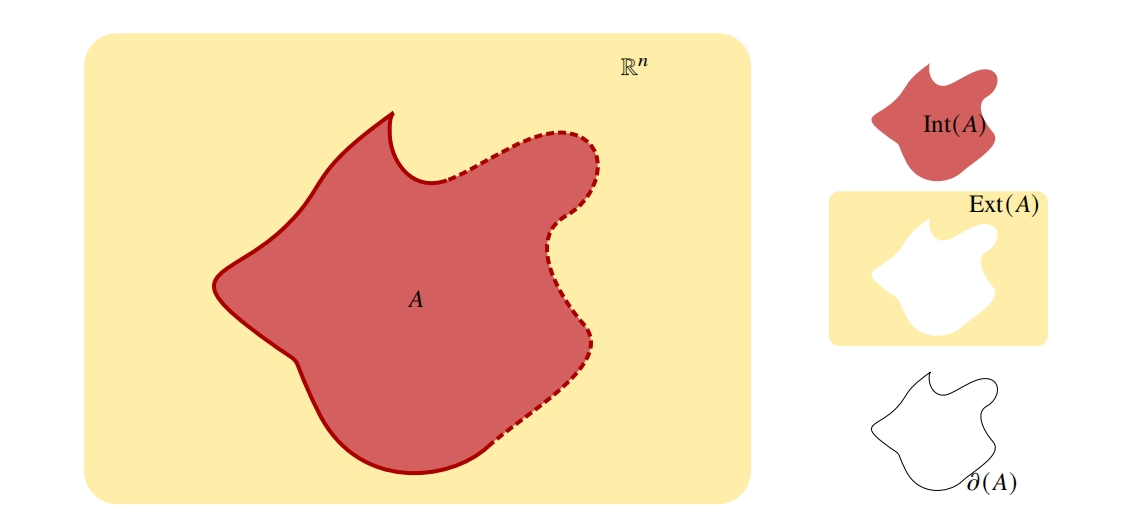
\includegraphics[width=0.6\textwidth]{figure/topological_space/int_ext_boundary.png}
    \caption{}
\end{figure}

By the following proposition, we can know closure and interior are closely related.

\begin{proposition}{}{}
   If $A=B^c$, then $\overline{A} = (\text{Int}(B))^c$.
\end{proposition}

\begin{proposition}{}{}
    (1) If $A\subset B$, then $\overline{A}\subset \overline{B}$;\\
    (2) $\overline{A}$ is the smallest closed subset of $X$ containing $A$;\\
    (3) $\overline{A}$ is the intersection of all closed sets of $X$ containing $A$;\\
    (4) $\overline{A}=A$ iff $A$ is closed;\\
    (5) $\overline{A\cup B}=\overline{A}\cup\overline{B}$;\\
    (6) $\overline{A\cap B}\subset \overline{A}\cap \overline{B}$.
\end{proposition}

\begin{example}{}{}
    Let $X=\{a,b,c,d,e\}$ and
    \begin{align*}
        \tau=\{X,\O,\{a\},\{c,d\},\{a,c,d\},\{b,c,d,e\}\}. 
    \end{align*} 
    Show that $\overline{\{b\}} = \{b,e\}$. 
\end{example}



\begin{definition}{}{}
    Let $A$ be a subset of a topological space $(X,\tau)$. Then $A$ is said to be dense in $X$ if $\overline{A}=X$.
    $X$ is said to be separable if there exists countable dense subset in $X$.
\end{definition}

\begin{proposition}{}{}
   Let $A$ be a subset of a topological space $(X,\tau)$. Then $A$ is dense in $X$ iff every non-empty open subset of $X$ intersects $A$ non-trivially, i.e.
   if $U\in \tau$ and $U\neq \O$ then $A\cap U\neq \O$. 
 \end{proposition}


\begin{example}{}{}
    $(X,\tau_d)$ is separable iff $X$ is countable. 
\end{example}
refer to \href{https://astarmathsandphysics.com/university-maths-notes/topology/2198-proof-that-a-discrete-space-is-separable-if-and-only-if-it-is-countable.html}{website proof}.


\begin{example}{}{}
    $(X,\tau_t)$ is separable. 
\end{example}
Let $A$ be a countably infinite subset of $X$. By example\ref{exa:limit point in trival topology}, 
$\overline{A}$ = $X$. Hence, $A$ is dense in $X$ and so $X$ is separable.
\begin{example}{}{}
    $(X,\tau_f)$ is separable.
\end{example}
    Let $A$ be a countably infinite subset of $X$. By example\ref{exa:limit point in cofinite topology}, 
    $\overline{A}$ = $X$. Hence, $A$ is dense in $X$ and so $X$ is separable.

\begin{example}{}{}
    $(X,\tau_c)$ is inseperable. 
\end{example}
    Let $A$ be a countably infinite subset of $X$.By example\ref{exa:limit point in cocountable topology},
    $\overline{A}$ = $A$. Hence, $X$ have no countably dense subset and so inseperable.

\begin{example}{}{}
    $(\R,\tau_e)$ is separable.
\end{example}
prove that $\overline{\Q}$=$\R$.


\subsection{Sequence convergence}
\begin{definition}{}{sequence convergence in topological space}
    Let $(X,\tau)$ be a topological space and $A$ a subset of $X$. Let $(x_n)_{n\in\N}$ be an infinite sequence in $A$.
    Then $(x_n)$ converages to the limit $x\in X$(denoted by $x_n\rightarrow x$) iff
    \begin{align*}
        \forall U\in \tau \text{ with }  x\in U \Rightarrow \{n\in \N:x_n\notin U\} \text{ is finite}.
    \end{align*}
    Or, 
    \begin{align*}
        \forall U\in \tau \text{ with }  x\in U \Rightarrow \exists N\in \N, \forall n>N, x_n\in U.
    \end{align*}
\end{definition}

In euclidean space,  the convergence point of a convergent sequence is unique and when $x$ is the limit point of the set $A$, there is a sequence $(x_n)$ in A, which converges to $x$. 
However, In general topological space, some difference appear.
\begin{proposition}{}{sequence convergence in cofinite topology}
    Let $(x_n)$ be a sequence which elements are different in $(R,\tau_f)$, then $\forall x\in X$, $x_n\rightarrow x$. 
\end{proposition}
\begin{proof}
    $\forall U\in \tau \text{ with }  x\in U \Rightarrow \{n\in \N:x_n\notin U\}= \{n\in \N:x_n\in U^c\} \text{ is finite}$.
\end{proof}
\begin{proposition}{}{sequence convergence in cocountable topology}
    Let $(x_n)$ be a sequence which elements are different in $(R,\tau_f)$, then
    \begin{align*}
        x_n\rightarrow x \Leftrightarrow \exists N\in\N, \forall n>N, x_n=x. 
    \end{align*}
\end{proposition}
\begin{proof}
    ($\Leftarrow$) clear by definition\ref{def:sequence convergence in topological space}
    \\
    ($\Rightarrow$) Consider the set $B:= \{x_n: x_n\neq x\}$. Since a sequence is countable, $B$ is countable. By example\ref{exa:limit point in cocountable topology}, B is closed.
    By construction, $x\notin B$, so $U=X\setminus B$ is an open set containing $x$. 
    But $x_n\rightarrow x$, so a tail of this sequence must lie in $X\setminus B$. Since $\{x_n\}\cap (X\setminus B)=\{x\}$, 
    this means that a tail of this sequence is constanst.  
\end{proof}

\section{Subspace}
\begin{definition}{}{}
    Let $A$ be a non-empty subset of a topological space $(X\,\tau)$. 
    The collection 
    \begin{align*}
        \tau_{A}=\{O\cap A: O\in \tau\}
    \end{align*}
    of subsets of $A$ is a topology on $A$ called the subspace topology
    (or the topology induced on $A$ by $\tau$). The topological space $(A,\tau_A)$ is said to be a subspace of $(X,\tau)$.
\end{definition}
Let's check that $\tau_A$ is indeed a topology on $A$.\\
(1) $A=X\cap A, \O = \O\cap A$, then $A,\O\in \tau_A$.\\
(2) If $U_{\alpha}\in \tau_A$, then $\cup_{\alpha}{U_\alpha} = \cup_{\alpha} (O_{\alpha}\cap A)=(\cup_{\alpha} O_{\alpha})\cap A\in\tau_A$.\\
(3) If $U_1,U_2\in\tau_A$, then $U_1\cap U_2 = (O_1\cap A)\cap (O_2\cap A)=(O_1\cap O_2)\cap A\in \tau_A$.

In the following content,  we follow the convention: a subset of topological Spaces is treated as a subspace. 
\par
Let $(X,\tau)$ be a topological space and $B\subseteq A\subseteq X$. Then
\begin{align*}
    (\tau_A)_B = & \{K\cap B:K\in \tau_A\} \\
        =  &\{(O\cap A)\cap B: O\in\tau\} \\
        =  &\{(O\cap B)\cap (A\cap B): O\in \tau\}\\
        \overset{B\subseteq A}{=}  &\{(O\cap B)\cap B: O\in \tau\}\\
        =  &\{(O\cap B): O\in \tau\}\\
        =  &\tau_B.
\end{align*}
Hence, there are two way to induce the topology on $B$: induced by the topology on $A$ or
induced by the topology on $X$.

\begin{example}{}{}
    Let $X=\{a,b,c,d,e,f\}$, 
    \begin{align*}
        \tau = \{X,\O, \{a\}, \{c,d\}, \{a,c,d\}, \{b,c,d,e,f\}\},
    \end{align*}
    and $A=\{b,c,e\}$. Then the subspace topology on $A$ is 
    \begin{align*}
        \tau_A = \{A,\O, \{c\}\}.
    \end{align*}
\end{example}


Consider the subset $[1,2]$ of $(\R,\tau_e)$. Then the topology on $[1,2]$ is 
\begin{align*}
    \tau = \{(a,b)\cap [1,2]: (a,b)\in \tau_e\}.
\end{align*}
\par
But here we see some surprising things happening; e.g.
$[1,\frac{3}{2})$ is certainly not an open set in $\R$, but $[1,\frac{3}{2})=(1,\frac{3}{2})\cap [1,2]$, is an open set in the subspace $[1,2]$.
\par
Also $(1,2]$ is not open in $\R$ but is open in $[1,2]$. Even $[1,2]$ is not open in $\R$, but is an open set in $[1,2]$.
\par
So whenever we speak of a set being open we must make perfectly clear in what space or what topology it is an open set. 

\begin{proposition}{}{closed intersection}
    Let $(X,\tau)$ be a topological space and $C\subset A\subset X$, then
    \begin{align*}
        C \text{ is closed in } A\Leftrightarrow C = A\cap V, \text{ where $V$ is closed in $X$}.  
    \end{align*}
\end{proposition}
\begin{proof}
    % \begin{align*}
    %     C \text{ is closed in } A &\Leftrightarrow A\setminus C \text{ is open in } A &\\
    %     & \Leftrightarrow \exists O\in \tau_{X}, \text{ s.t. } A\setminus C = O\cap A &\\
    %     & \Leftrightarrow \exists O\in \tau_{X}, C && = A\setminus(O\cap A) = (A\setminus O) \cup (A\setminus A) = &\\
    %     & &(A\setminus O) \cup \O = A\setminus O\\
         
    % \end{align*}

    \begin{align*}
        C \text{ is closed in } A &\Leftrightarrow A\setminus C \text{ is open in } A\\
         &\Leftrightarrow \exists O\in \tau_{X}, \text{ s.t. } A\setminus C = O\cap A\\
         &\Leftrightarrow \exists O\in \tau_{X}, C= A\setminus(O\cap A) \\
         &\quad\quad = (A\setminus O) \cup (A\setminus A)\\
         &\quad\quad = (A\setminus O) \cup \O = A\setminus O\\
         &\quad\quad = (A\cap X)\setminus O\\
         &\quad\quad = A\cap (X\setminus O)\\
         &\quad\quad = A\cap V, \text{ where $V$ is closed in $X$.}
        \end{align*}
\end{proof}

\begin{proposition}{}{}
    Let $(X,\tau)$ be a topological space, $B\subset A\subset X$, then\\
    (1) If $B$ is open(closed) in $X$, then $B$ is open(closed) in $A$;\\
    (2) If $A$ is open(closed) in $X$ and $B$ is open(closed) in $A$, then $B$ is open(closed) in $X$.
\end{proposition}
\begin{proof}
    (1) We know that $B=B\cap A$. If $B=O$ , then $B = O\cap A$ and so $B$ is open in $A$. 
    If $B$ is closed in $X$, by proposition\ref{prop:closed intersection}, $B=X\cap V$, where $V$ is closed in $X$. 
    Then $B=B\cap A = (X\cap V)\cap A = (X\cap A)\cap V$, by by proposition\ref{prop:closed intersection}, $B$ is closed in $A$.\\
    (2) If $B = O_1\cap A$ and $A=O_2$ , then $B=O_1\cap O_2\in \tau$ and so $B$ is open in $X$.
    If $A$ is closed in $X$ and $B$ is closed in $A$, then $A = X\cap V_1, B=A\cap V_2$, where $V_1,V_2$ is closed in $X$.
    Then, $B = X\cap (V_1\cap V_2)$. As $V_1\cap V_2$ is closed in $X$, $B$ is closed in $X$. 
\end{proof}

\section{Reference}
\begin{itemize}
    \item \href{https://www.ms.uky.edu/~guillou/F14/551Notes-Week4.pdf}{lecture notes from uky}
\end{itemize}
\section{Exercise}


\chapter{Continuous Mappings and Homeomorphisms}\label{1_2}

\section{Continuous Mappings}
We are already familiar with the notion of a continuous function from $\R$ to $\R$.
\par
A function $f:\R\rightarrow \R$ is said to be continuous at $x_0\in \R$ iff each positive real number $\epsilon$, 
there exists a positive real number $\delta$ such that $|f(x)-f(x_0)|<\epsilon$ when $|x-x_0|<\delta$. 
\par
It is not all obvious how to generalize this definition to general topological spaces where we do not have 
"absolute value" or "subtraction". So we shall seek another(equivalent) definition of continuity which lends itself more to 
generalization. 

It is easily seen that: $f:\R\rightarrow \R$ is continuous at $x_0\in\R$ iff for each interval $(f(x_0)-\epsilon, f(x_0)+\epsilon)$, 
for $\epsilon>0$, there exists a $\delta>0$ such that $f(x)\in(f(x_0)-\epsilon, f(x_0)+\epsilon)$ for all $x\in(x_0-\delta,x_0+\delta)$.
\par
This definition is an improvement since it does not involve the concept "absolute value" but it still involves "substraction". 
The next definition shows how to avoid substraction.

\begin{definition}{}{continuity definition}
    Let $(X,\tau)$ and $(Y,\tau')$ be topological spaces and $f$ a function from $X$ into $Y$.
    Then $f$ is continuous at $x_0\in X$ iff
    for each $U\in \tau'$ containing $f(x_0)$, there exists $K\in\tau$ containing $x_0$, such that $f(K)\subseteq U$.
\end{definition}
Use neighborhood to describe
\begin{proposition}{}{}
    Let $(X,\tau)$ and $(Y,\tau')$ be topological spaces and $f$ a function from $X$ into $Y$.
    Then $f$ is continuous at $x_0\in X$ iff for any neighborhood $N$ of $f(x_0)$ in $Y$, $f^{-1}$ is the neighborhood of $x_0$.
\end{proposition}
\begin{proof}
    
\end{proof}
\begin{definition}{}{}
    Let $(X,\tau)$ and $(Y,\tau')$ be topological spaces and $f$ a function from $X$ into $Y$.
    Then $f$ is continuous iff for each $x_0\in X$ and for each $U\in \tau'$ containing $f(x_0)$, 
    there exists $K\in\tau$ containing $x_0$, such that $f(K)\subseteq U$.
\end{definition}

As in analysis, continuity is a local concept. 
\begin{proposition}{}{}
    Let $(X,\tau)$ and $(Y,\tau')$ be topological spaces and $f$ a function from $X$ into $Y$ , $A$ a subset of $X$ and $x_0\in A$.
    We define the restriction of $f$ on $A$ as $f_A = f|A:A\rightarrow Y$, then\\
    (1) If $f$ is continuous at $x_0$, then $f_A$ is continuous at $x_0$.\\
    (2) When $A$ is open in $X$, if $f_A$ is continuous at $x_0$, then $f$ is continuous at $x_0$.
\end{proposition}

\begin{proof}
    (1) We need to prove for each $U\in \tau'$ with $f_A(x_0)\in U$, there exists $O\in \tau_A$ with $x_0\in O$, $f_A(O)\subseteq U$.
    $f$ is continuous at $x_0$ and $x_0\in A$, then for each $U\in \tau'$ with $f(x_0)=f_A(x_0)\in U$, there exists $K\in \tau$ with $x_0\in K$, $f(K)\subseteq U$.
    Since $A\cap K\in \tau_A$ with $x_0\in A\cap K$ and $f_A(A\cap K) = f(A\cap K)\subseteq f(A)\cap f(K)\subseteq Y\cap U= U$. Hence, $f_A$ is continuous at $x_0$.
    \par
    (2) $f_A$ is continuous at $x_0$, then for each $U\in\tau'$ containing $f_A(x_0)=f(x_0)$, there exists $(K\cap A)\in \tau_A$($K\in\tau$) containing $x_0$, 
    such that $f_A(K\cap A)\subseteq U$. Since $A\in \tau$, $K\cap A\in \tau$ and $f(A\cap K)=f_A(A\cap K)\subset U$. Hence, $f$ is continuous at $x_0$. 
\end{proof}


\begin{definition}{}{}
    Let $f$ be a function from a set $x$ into a set $Y$. If $S$ is any subset of $Y$, 
    then the set $f^{-1}(S)$ is defined by
    \begin{align*}
        f^{-1}(S) = \{x:x\in X \text{ and } f(x)\in S\}.
    \end{align*}
    Then subset $f^{-1}(S)$ of $X$ is said to be the inverse image of $S$.
\end{definition}
\begin{remark}
    Note that an inverse function of $f$ exists iff $f$ is bijective. 
    But the inverse image of any subset of $Y$ exists even if $f$ is neither one-to-one nor onto.
\end{remark}

\begin{proposition}{}{}
    Let $f$ be a mapping of a topological space $(X,\tau)$ into a topological space $(Y,\tau')$. Then the following conditions are equivalent:\\
    (1) $f$ is continuous;\\
    (2) for each $U\in\tau'$, $f^{-1}(U)\in \tau$;\\
    (3) for each closed set $V$ in $Y$, $f^{-1}(Y)$ is closed in $X$.
\end{proposition}

\begin{proof}
    
\end{proof}

In $(\R,\tau_e)$, we can use sequence convergence to characterize continuity, 
but in general topological space, we cannot do this.
\begin{proposition}{}{continuity means sequentially continous}
    $f:X\rightarrow Y$ is continuous at $x_0\in X$, then $x_n\rightarrow x_0$ implies $f(x_n)\rightarrow f(x_0)$.
\end{proposition}
\begin{proof}
    $f$ is continous at $x_0\in X$ and $x_n\rightarrow x_0$, 
    then $\forall U\in\tau_Y$ containing $f(x_0)$, 
    there exists $K\in\tau_X$ containing $x_0$ such that $f(K)\subseteq U$.
    Since $x_n\rightarrow x_0$, $\exists N\in\N$, $\forall n>N$, $x_n\in K$, then $f(x_n)\in f(K)\subseteq U$.
    So $f(x_n)\rightarrow f(x_0)$.
\end{proof}
However, the inverse proposition is not true. 
Let $f:X\rightarrow Y$ be injective, $X$ be a uncountable space with $\tau_c$ and $Y$ be a discrete space.
Then, by proposition\ref{prop:sequence convergence in cocountable topology}, 
When $x_n\rightarrow x_0$ in $X$, $\exists N\in N$, $\forall n>N$, $x_n=x$, 
then $f(x_n)=f(x)$ and so $f(x_n)\rightarrow f(x)$.
But $f$ is not continuous at $x_0$, because for $U=\{f(x_0)\}\in \tau_Y$ containing $f(x_0)$, 
$\forall K\in \tau_X$ containing $x_0$, $f(K)\supset \{f(x_0)\}$ as $f$ is injective and $K\supset \{x_0\}$.


\section{The properties of continuous mapping}

Firstly, we introduce some simple and common continuous mappings.
\begin{proposition}{}{}
    Identity mapping $\text{id}:X\rightarrow X$ is continuous.
\end{proposition}

\begin{definition}{}{Inclusion mapping}
        Let $X$ be a topological space and $A\subset X$. 
        Then inclusion mapping $i_A:A\rightarrow X$ is the mapping defined as:
        \begin{align*}
            i_A:A\rightarrow X: \forall x\in A:i_{A}(x)=x
        \end{align*}
\end{definition}

\begin{proposition}{}{}
    Let $X$ be a topological space and $A\subset X$. 
    Then inclusion mapping $i_A:A\rightarrow X$ is continuous.
\end{proposition}

\begin{proof}
    For any open set $U$ in $X$, $i^{-1}(U)=U\cap A$ is open in $A$.
\end{proof}

\section{Homemorphism}

\begin{definition}{}{}
    Let $(X,\tau)$ and $(Y,\tau')$ be topological spaces, 
    and let $f:X\rightarrow Y$ be a bijection. 
    $f$ is said to be a homeomorphism if $f$ is continous and its inverse $f^{-1}$ is continous.\\
    In this case we say that $(X,\tau)$ and $(Y,\tau')$ are homeomorphism, and write $(X,\tau)\cong (Y,\tau')$, or
    more often simply $X\cong Y$ if the topologies are understood from context.
\end{definition}

\begin{proposition}{}{}
    Let $(X,\tau)$ and $(Y,\tau')$ be a topological spaces, and let $f:X\rightarrow Y$ be a bijection, 
    Then the following are equivalent.\\
    (1) $f$ is a homeomorphism.\\
    (2) $f$ is continous and open.\\
    (3) $f$ is continuous and closed.\\
    (4) $U\subset X$ is open iff $f(U)\subset Y$ is open.
\end{proposition}

\begin{definition}
    Let $X$ and $Y$ be topological spaces. 
    Suppose $f:X\rightarrow Y$ is an injective continous mapping. 
    If the function $f':X\rightarrow f(X)$ obtained by restricting the range of $f$ is a homeomorphism, 
    then the map $f:X\rightarrow Y$ is called a topological embedding.
\end{definition}

\section{Exercise}

\begin{exercise}{}{}
    Let $f$ be a mapping from $X$ to $Y$, the following statements are equivalent:\\
    (1) $f$ is continous;\\
    (2) $\forall A\subseteq X$, $f(\overline{A})\subset \overline{f(A)}$;\\
    (3) $\forall B\subseteq Y$, $\overline{f^{-1}(B)}\subset f^{-1}(\overline{B})$.
\end{exercise}

\begin{proof}
    (1)$\Rightarrow$(2): $f$ is continous. Since $\overline{f(A)}$ is closed in $Y$, 
    then $f^{-1}(\overline{f(A)})$ is closed in $X$. Since $f(A)\subseteq \overline{f(A)}$, 
    $A\subseteq f^{-1}(\overline{f(A)})$. Since $\overline{A}$ is the smallest closed set containing $A$, 
    $\overline{A}\subseteq f^{-1}(\overline{f(A)})$. Then, $f(\overline{A})\subseteq f(f^{-1}(\overline{f(A)}))\subseteq \overline{f(A)}$.

\end{proof}

\begin{exercise}{}{}
    $f:X\rightarrow Y$ is called open(closed) mapping, if $f(X)$ is open(closed). 
    Illustrate that open mapping may not be closed mapping and vice versa.
\end{exercise}
\begin{proof}
    
\end{proof}

\begin{exercise}
    If $f:X\rightarrow Y$ is bijective, then
    \begin{align*}
        f \text{ is open mapping }\Leftrightarrow f\text{ is closed mapping }\Leftrightarrow f^{-1} \text{ is continuous}.
    \end{align*}
\end{exercise}

\begin{proof}
    $\forall U\in\tau_X$,
    \begin{align*}
        f(U)\in \tau_Y \Leftrightarrow & Y\setminus f(U) \text{ is closed }\\
                                \overset{f \text{ is bijective }}{\Leftrightarrow} & f(X\setminus U) \text{ is closed } \\
                                \Leftrightarrow & f \text{ is closed mapping}.
    \end{align*}
    Since $f$ is bijective, $f^{-1}$ exists. As $f$ is open mapping, $f^{-1}$ is continuous.
\end{proof}

\begin{remark}
    From this exercise, we can know if $f$ is bijective, continuous and open, then $f$ is homeomorphism.
\end{remark}

\section{Reference}

\begin{itemize}
    \item \href{https://raphaeltinarrage.github.io/files/EMAp/Lesson2.pdf}{Homeomorphisms}
    \item 
\end{itemize}



\newcommand{\ob}{\overline{\mathcal{B}}}
\chapter{Topological basis and Product Space}\label{chp:1_3}


\section{Topological basis}
Let's recall the euclidean topology in $\R$, 
\begin{align*}
    \tau_e = \{U : U=\cup_{(a,b)\in I} (a,b), a<b\in \R, I \text{ is a collection of open interval}\}.
\end{align*}
It seems like the entire collection of sets
in $\tau_e$ can be specified by declaring that just the usual open intervals are open. Once these
“special sets” are known to be open, we get all the other sets for free by taking unions.
These special collections of sets are called bases of topologies.

\begin{definition}{}{basis for given topology definition}
    Let $(X,\tau)$ be a topological space. 
    A collection $\mathcal{B}$ of subsets of $X$ is said to be a basis for the topology $\tau$
    if for each $U\in \tau$, $U=\cup_{B\in I} B$, where $I\subseteq \mathcal{B}$.
\end{definition}

If we construct a set $\ob=\{U_{B\in I}B: I \subseteq \mathcal{B}\}$, 
then we can get a improved definition. 

\begin{definition}{}{basis for given topology definition}
    Let $(X,\tau)$ be a topological space. 
    A collection $\mathcal{B}$ of subsets of $X$ is said to be a basis for the topology $\tau$
    if $\ob=\tau$.
\end{definition}

\begin{proposition}{}{}
    Let $(X, \tau)$ be a topological space.
     A collection $\mathcal{B} \subseteq \mathcal{P}(X)$ is a
basis for $\tau$ if and only if\\
(1) $\mathcal{B} \subseteq \tau$,\\
(2) for any $U \in \tau$ and any $x \in U$, there exists $B \in \mathcal{B}$ such that $x \in B \subseteq U$.
\end{proposition}

\begin{proof}
    ($\Rightarrow$): Suppose $\ob=\tau$, then $\mathcal{B}\subseteq \ob\subseteq \tau$. 
    Since $\tau\subseteq \ob$, then take $B=U$, $x\in B\subseteq U$.
    \\
    ($\Leftarrow$): (1) implies $\ob\subseteq \tau$, 
    (2) implies $U\subseteq \cup_{B_x}B_x\subseteq U$ and so $U=\cup_{B_x}B_x\in \ob$. 
    Hence, $\ob\subseteq \tau$ and so $\ob=\tau$.
\end{proof}

\begin{example}{}{}
    $\mathcal{B}=\{(a,b):a,b\in\R,a<b\}$ is a basis for $(\R,\tau_e)$.
\end{example}

\begin{example}{}{}
    $\mathcal{B}=\{\{x\}:x\in X\}$ is a basis for $(X,\tau_s)$. 
\end{example}

Observe that $\tau=\mathcal{P}(X)$ is also a basis for the discrete topology on $X$. 
Therefore, there can be many different bases for the same topology. indeed if $\mathcal{B}$ is a basis for a topology $\tau$ on a set $X$ and $\mathcal{B}_1$ is a collections of subsets of $X$ such that $\mathcal{B}\subseteq \mathcal{B}_1\subseteq \tau$, then $\mathcal{B}_1$ is also a basis for $\tau$.


The above content show us when $\mathcal{B}$ is basis for a given topology in $X$. 
Now we consider when $\mathcal{B}$ is basis for a topology in $X$.

\begin{proposition}{}{}
    Let $X$ be a non-empty set and $\ob$ be a collection of subsets of $X$. Then $\mathcal{B}$ is a basis for a topology on $X$ iff
    $\overline{B}$ is a topology.
\end{proposition}


\begin{proposition}{Basis for a topology}{}
    Let $X$ be a non-empty set and $\mathcal{B}$ be a collection of subsets of $X$. Then $\mathcal{B}$ is a basis for a topology on $X$ iff $\mathcal{B}$ has the following properties:\\
    (1) $X=\cup_{B\in \mathcal{B}}B$, and\\
    (2) for any $B_1,B_2\in \mathcal{B}$, $B_1\cap B_2=\cup_{B\in I}B$, where $I\subseteq\mathcal{B}$.
\end{proposition}

\begin{proof}
($\Rightarrow$): $\ob$ is a topology, then $X\in \ob$ and so $X=\cup_{B\in I}B$.
Since $B\in\mathcal{B}$ is contained in $X$, $X\subseteq \cup_{B\in\mathcal{B}}\subseteq X$. Hence, $X=\cup_{B\in\mathcal{B}}B$.
If $B_1,B_2\in\mathcal{B}$, then $B_1,B_2\in\ob$ and so $B_1,B_2$ is open. Then $B_1\cap B_2$ is open and so contained in $\ob$. 

($\Leftarrow$): We should show that $\ob$ is a topology. By (1), $X\in\ob$. 
$\O$ is the empty union of members in $\ob$. Hence, $\O\in\ob$. For $U_J=\{U\in J: J\subseteq\ob\}$, $U$ is the union of members in $\mathcal{B}$.
Then $\cup_{U\in U_J} U$ is the union of members in $\mathcal{B}$ and so belong to $\ob$. 
If $U_1,U_2\in \ob$, then $U_1=\cup_{B_1\in I_1}B_1, U_2=\cup_{B_2\in I_2}B_2$.
Then $U_1\cap U_2 = (\cup_{B_1\in I_1}B_1)\cap (\cup_{B_2\in I_2}B_2)=\cup_{B_1\in I_1}(B_1\cap (\cup_{B_2\in I_2}B_2))= \cup_{B_1\in I_1,B_2\in I_2}(B_1\cap B_2)$. 
By (2), $B_1\cap B_2$ is the union of members in $\mathcal{B}$, thus $U_1\cap U_2$ is the union of members in $\mathcal{B}$ and so contained in $\mathcal{B}$.
Hence, $\ob$ is a topology.
\end{proof}

\textcolor{red}{Haven't done! Add the content about basis for a given topology.}

\section{Product space}


\part{Topology Invariant}
\chapter{The Axioms of Countablity and Separation}\label{chp:axioms countablity & separation}



\chapter{Compactness}\label{chp:compactness}

\begin{theorem}{}{}
    In metric space, compactness and sequential compactness are equivalent.
\end{theorem}




\begin{remark}
    In general topology space, compactness and sequential compactness are not equivalent. You can refer to 
\href{https://math.stackexchange.com/questions/152447/compactness-sequentially-compact}{answer in mathexchange}.
\end{remark}



\section{Reference}

\begin{itemize}
    \item \href{https://people.clas.ufl.edu/mjury/files/sequential_compactness_notes.pdf}{lecture note from Florida}
    \item \href{https://www.umsl.edu/~siegelj/SetTheoryandTopology/Compact2.html}{The Lebesgue Number of a Covering}
\end{itemize}





\end{spacing}
\end{document}